%%%%%%%%%%%%%%
%% Run LaTeX on this file several times to get Table of Contents,
%% cross-references, and citations.

%% If you have font problems, you may edit the w-bookps.sty file
%% to customize the font names to match those on your system.

%% w-bksamp.tex. Current Version: Feb 16, 2012
%%%%%%%%%%%%%%%%%%%%%%%%%%%%%%%%%%%%%%%%%%%%%%%%%%%%%%%%%%%%%%%%
%
%  Sample file for
%  Wiley Book Style, Design No.: SD 001B, 7x10
%  Wiley Book Style, Design No.: SD 004B, 6x9
%
%
%  Prepared by Amy Hendrickson, TeXnology Inc.
%  http://www.texnology.com
%%%%%%%%%%%%%%%%%%%%%%%%%%%%%%%%%%%%%%%%%%%%%%%%%%%%%%%%%%%%%%%%

%%%%%%%%%%%%%
% 7x10
%\documentclass{wileySev}

% 6x9
\documentclass{wileySix}

\usepackage{graphicx}
\usepackage{listings}
\usepackage{float}
\usepackage[urlcolor=blue,colorlinks=true]{hyperref}
\usepackage{color}

\definecolor{codegreen}{rgb}{0,0.6,0}
\definecolor{codegray}{rgb}{0.5,0.5,0.5}
\definecolor{codepurple}{rgb}{0.58,0,0.82}
\definecolor{backcolour}{rgb}{0.95,0.95,0.92}

\lstdefinestyle{mystyle}{
    backgroundcolor=\color{backcolour},
    commentstyle=\color{codegreen},
    keywordstyle=\color{magenta},
    numberstyle=\tiny\color{codegray},
    stringstyle=\color{codepurple},
    basicstyle=\footnotesize,
    breakatwhitespace=false,
    breaklines=true,
    captionpos=b,
    keepspaces=true,
    numbers=left,
    numbersep=5pt,
    showspaces=false,
    showstringspaces=false,
    showtabs=false,
    tabsize=2,
    language=sh
}

\lstset{style=mystyle}

%%%%%%%
%% for times math: However, this package disables bold math (!)
%% \mathbf{x} will still work, but you will not have bold math
%% in section heads or chapter titles. If you don't use math
%% in those environments, mathptmx might be a good choice.

% \usepackage{mathptmx}

% For PostScript text
\usepackage{w-bookps}

%%%%%%%%%%%%%%%%%%%%%%%%%%%%%%%%%%%%%%%%%%%%%%%%%%%%%%%%%%%%%%%%
%% Other packages you might want to use:

% for chapter bibliography made with BibTeX
% \usepackage{chapterbib}

% for multiple indices
% \usepackage{multind}

% for answers to problems
% \usepackage{answers}

%%%%%%%%%%%%%%%%%%%%%%%%%%%%%%
%% Change options here if you want:
%%
%% How many levels of section head would you like numbered?
%% 0= no section numbers, 1= section, 2= subsection, 3= subsubsection
%%==>>
\setcounter{secnumdepth}{3}

%% How many levels of section head would you like to appear in the
%% Table of Contents?
%% 0= chapter titles, 1= section titles, 2= subsection titles,
%% 3= subsubsection titles.
%%==>>
\setcounter{tocdepth}{2}

%% Cropmarks? good for final page makeup
%% \docropmarks

%%%%%%%%%%%%%%%%%%%%%%%%%%%%%%
%
% DRAFT
%
% Uncomment to get double spacing between lines, current date and time
% printed at bottom of page.
% \draft
% (If you want to keep tables from becoming double spaced also uncomment
% this):
% \renewcommand{\arraystretch}{0.6}
%%%%%%%%%%%%%%%%%%%%%%%%%%%%%%

%%%%%%% Demo of section head containing sample macro:
%% To get a macro to expand correctly in a section head, with upper and
%% lower case math, put the definition and set the box
%% before \begin{document}, so that when it appears in the
%% table of contents it will also work:

\newcommand{\VT}[1]{\ensuremath{{V_{T#1}}}}

%% use a box to expand the macro before we put it into the section head:

\newbox\sectsavebox
\setbox\sectsavebox=\hbox{\boldmath\VT{xyz}}

%%%%%%%%%%%%%%%%% End Demo


\begin{document}


\booktitle{SIG (Sistem Informasi Geografis)}
\subtitle{Semester 5}

\authors{D4TI3B\\
\affil{Angkatan 2017}
%Floyd J. Fowler, Jr.\\
%\affil{University of New Mexico}
}

\offprintinfo{SIG (Sistem Informasi Geografis), First Edition}{D4TI3A}

%% Can use \\ if title, and edition are too wide, ie,
%% \offprintinfo{Survey Methodology,\\ Second Edition}{Robert M. Groves}

%%%%%%%%%%%%%%%%%%%%%%%%%%%%%%
%%
\halftitlepage

%\titlepage


\begin{copyrightpage}{2019}
\input{info/copyrightpage}
\end{copyrightpage}

\dedication{`Jika Kamu tidak dapat menahan lelahnya belajar,
Maka kamu harus sanggup menahan perihnya Kebodohan.'
~Imam Syafi'i~}

\begin{contributors}
\input{info/contributors}
\end{contributors}

\contentsinbrief
\tableofcontents
\listoffigures
\listoftables
\lstlistoflistings


\begin{foreword}
\input{info/foreword}
\end{foreword}

\begin{preface}
\input{info/preface}
\end{preface}


\begin{acknowledgments}
\input{info/acknowledgments}
\end{acknowledgments}

\begin{acronyms}
\input{info/acronyms}
\end{acronyms}

\begin{glossary}
\input{info/glossary}
\end{glossary}

\begin{symbols}
\input{info/symbols}
\end{symbols}

\begin{introduction}
\input{info/introduction}
\end{introduction}

%%%%%%%%%%%%%%%%%% Isi Buku %%%%%%%%%%%%%%%%%%
\chapter{Tugas Pertama}
\input{chapters/tugas1/1174xxx}
\input{chapters/tugas1/1174039}
\input{chapters/tugas1/1174042}
\section{Alit Fajar Kurniawan (1174057)}
\subsection{Membaca file shp dengan pyshp}
\begin{enumerate}
	\item 
	\lstinputlisting{src/2/1174057/soal1.py}
	\begin{figure}[H]
		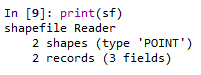
\includegraphics[width=12cm]{figures/1174057/fajar1.PNG}
		\centering
		\caption{Gambar no. 1}
	\end{figure}
	
	\item 
	\lstinputlisting{src/2/1174057/soal2.py}
	\begin{figure}[H]
		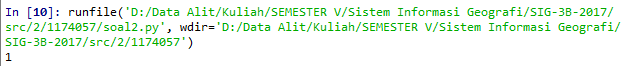
\includegraphics[width=12cm]{figures/1174057/fajar2.PNG}
		\centering
		\caption{Gambar no. 2}
	\end{figure}
	
	\item 
	\lstinputlisting{src/2/1174057/soal3.py}
	\begin{figure}[H]
		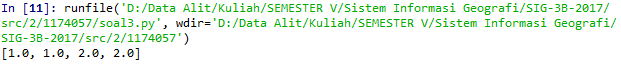
\includegraphics[width=12cm]{figures/1174057/fajar3.PNG}
		\centering
		\caption{Gambar no. 3}
	\end{figure}
	
	\item 
	\lstinputlisting{src/2/1174057/soal4.py}
	\begin{figure}[H]
		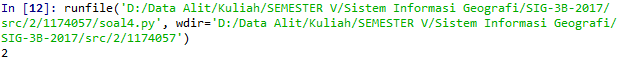
\includegraphics[width=12cm]{figures/1174057/fajar4.PNG}
		\centering
		\caption{Gambar no. 4}
	\end{figure}
	
	\item 
	\lstinputlisting{src/2/1174057/soal5.py}
	\begin{figure}[H]
		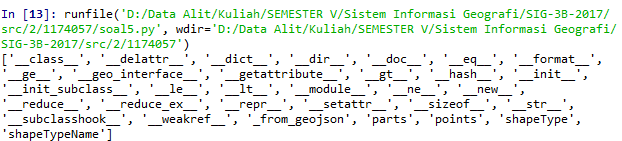
\includegraphics[width=12cm]{figures/1174057/fajar5.PNG}
		\centering
		\caption{Gambar no. 5}
	\end{figure}
	
	\item 
	\lstinputlisting{src/2/1174057/soal6.py}
	\begin{figure}[H]
		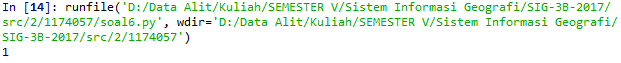
\includegraphics[width=12cm]{figures/1174057/fajar6.PNG}
		\centering
		\caption{Gambar no. 6}
	\end{figure}
	
	\item 
	\lstinputlisting{src/2/1174057/soal7.py}
	\begin{figure}[H]
		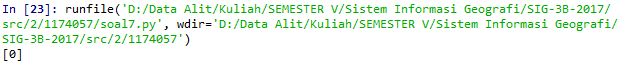
\includegraphics[width=12cm]{figures/1174057/fajar7.PNG}
		\centering
		\caption{Gambar no. 7}
	\end{figure}
	
	\item 
	\lstinputlisting{src/2/1174040/8.py}
	\begin{figure}[H]
		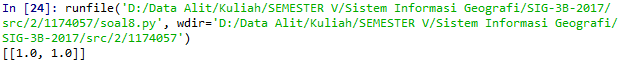
\includegraphics[width=12cm]{figures/1174057/fajar8.PNG}
		\centering
		\caption{Gambar no. 8}
	\end{figure}
	
	\item 
	\lstinputlisting{src/2/1174057/soal9.py}
	\begin{figure}[H]
		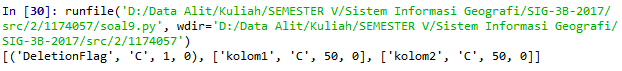
\includegraphics[width=12cm]{figures/1174057/fajar9.PNG}
		\centering
		\caption{Gambar no. 9}
	\end{figure}

    \item 
	\lstinputlisting{src/2/1174057/soal10.py}
	\begin{figure}[H]
		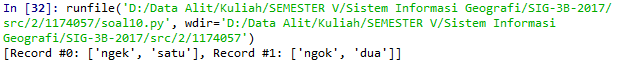
\includegraphics[width=12cm]{figures/1174057/fajar10.PNG}
		\centering
		\caption{Gambar no. 10}
	\end{figure}

	\item 
	\lstinputlisting{src/2/1174057/soal11.py}
	\begin{figure}[H]
		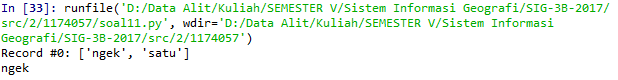
\includegraphics[width=12cm]{figures/1174057/fajar11.PNG}
		\centering
		\caption{Gambar no. 11}
	\end{figure}
\end{enumerate}

\subsection{Link}
\href{https://www.youtube.com/watch?v=PxCZFZzLivM}{Video ni}
\input{chapters/tugas1/1174035}
\input{chapters/tugas1/1174040}
\input{chapters/tugas1/1174043}
\section{Dika Sukma Pradana(1174050)}
\subsection{LeafletJs bersama Map Proxy}
\begin{enumerate}
 \item Sesuaikan direktorinya dengan milik kita
    \hfill\break
    \begin{figure}[H]
		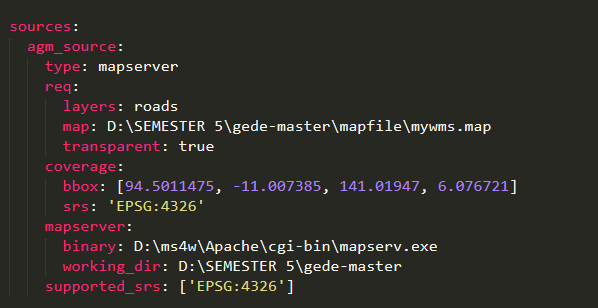
\includegraphics[width=12cm]{figures/1174050/tugas5/2.PNG}
		\centering
		\caption{Penyesuaian Direktori}
	\end{figure}
    \item Run Map Proxy dengan perintah mapproxy-util serve-develop agm.yaml
    \hfill\break
    \begin{figure}[H]
		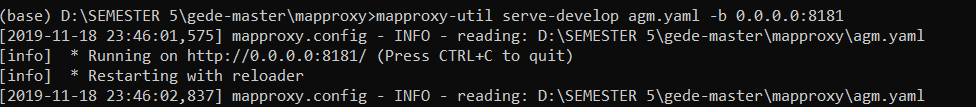
\includegraphics[width=12cm]{figures/1174050/tugas5/1.PNG}
		\centering
		\caption{Run MapProxy}
	\end{figure}
    \item Buka file basic.html di chrome sesuai direktorinya
    \hfill\break
    \begin{figure}[H]
		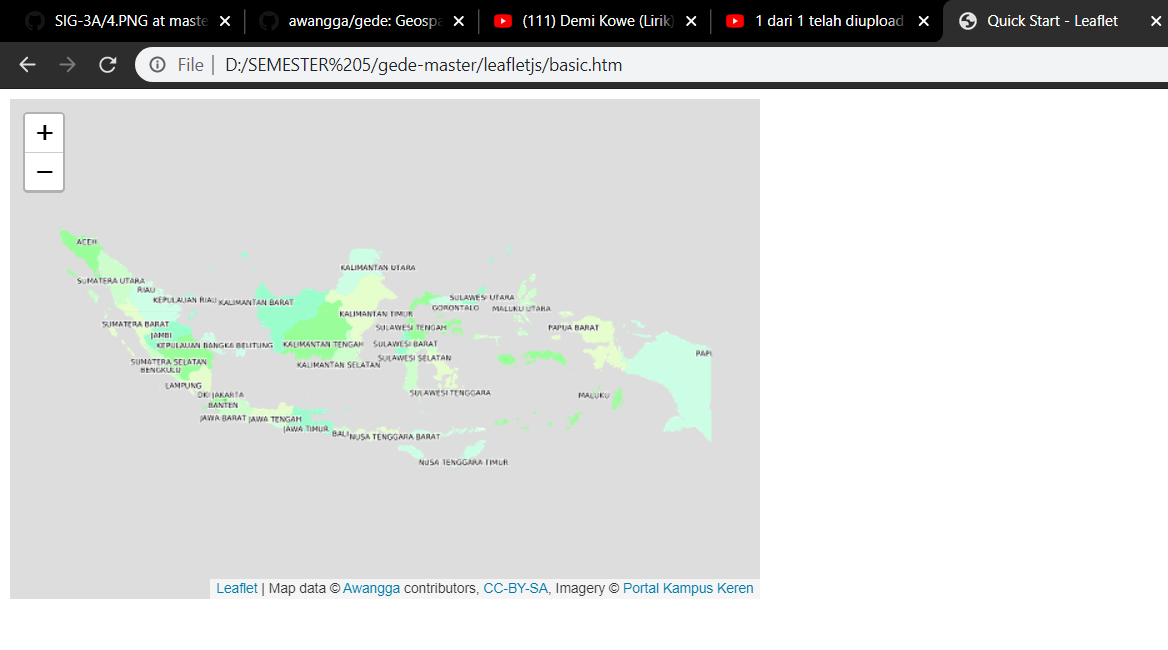
\includegraphics[width=12cm]{figures/1174050/tugas5/3.PNG}
		\centering
		\caption{Buka di Chrome}
	\end{figure}
    \item Pada file marker.html sudah ditambahkan marker pada daerah tertentu
    \hfill\break
    \begin{figure}[H]
		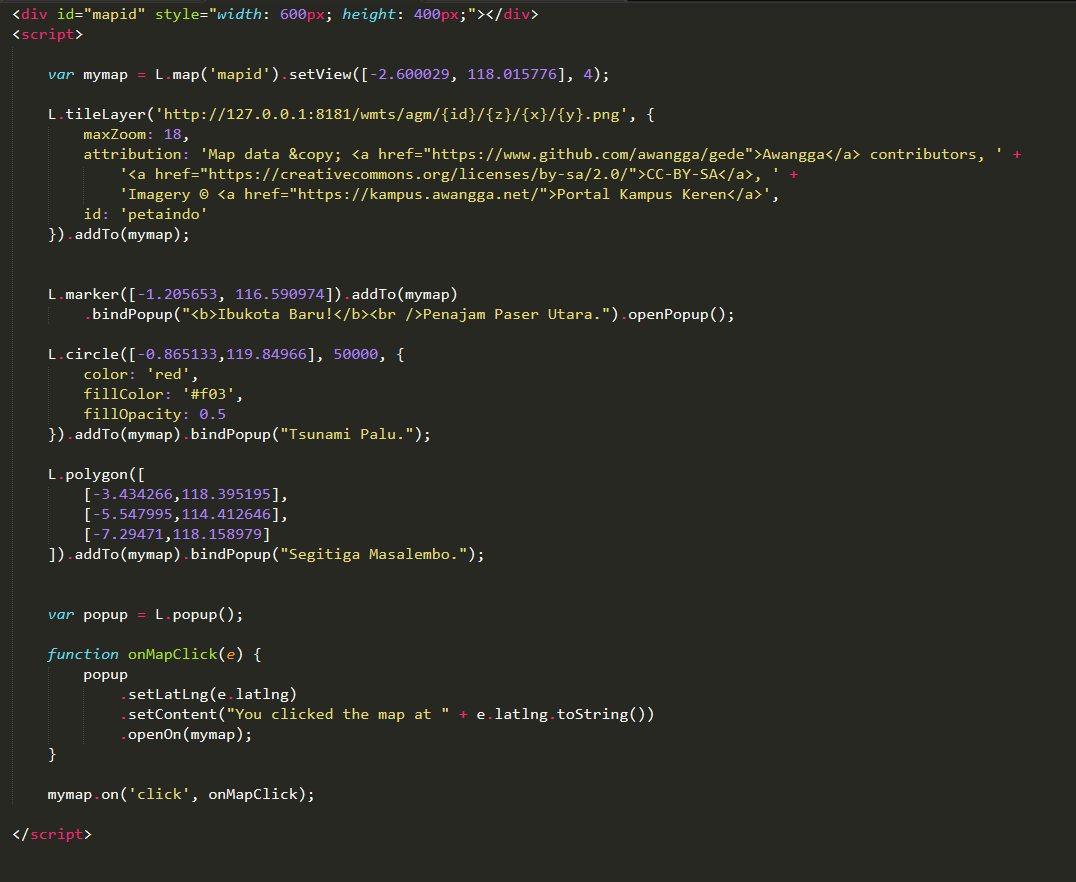
\includegraphics[width=12cm]{figures/1174050/tugas5/4.PNG}
		\centering
		\caption{Tambah Marker}
	\end{figure}
    \item Buka marker.html di browser
    \hfill\break
    \begin{figure}[H]
		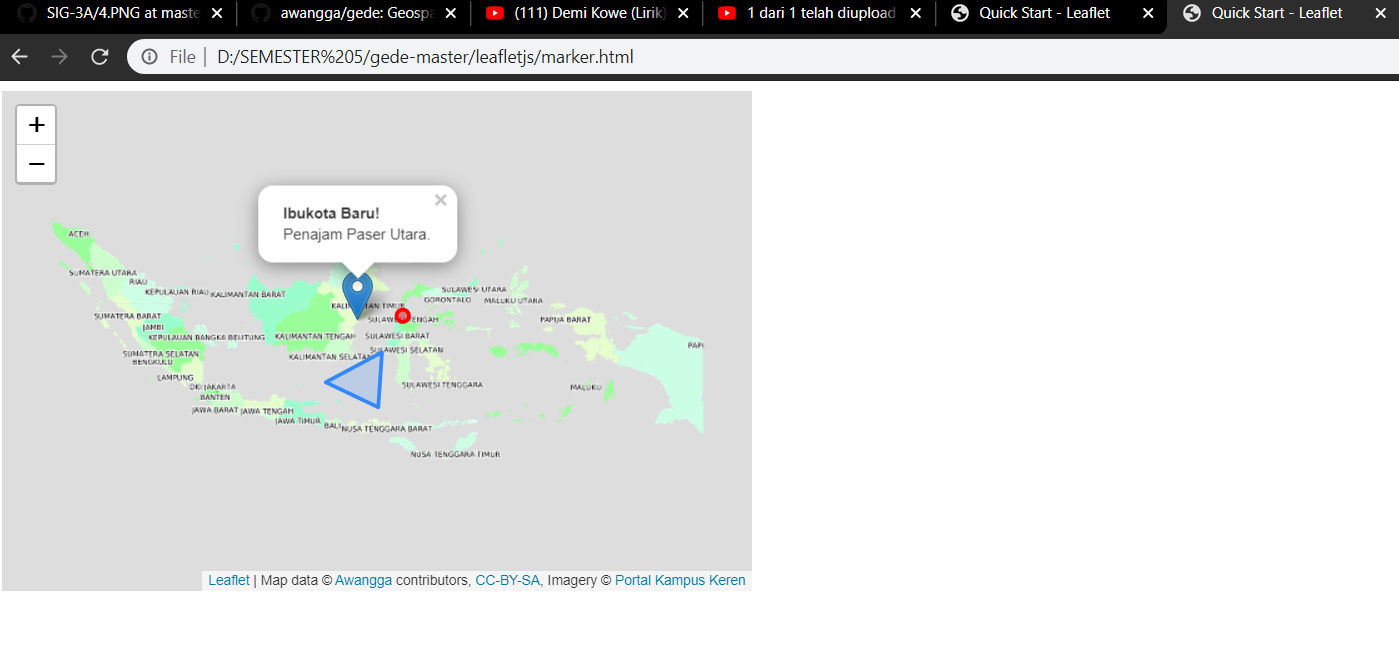
\includegraphics[width=12cm]{figures/1174050/tugas5/5.PNG}
		\centering
		\caption{Tampilan di Browser}
	\end{figure}
\end{enumerate}
\subsection{Link Youtube}
\href{https://youtu.be/1eIGj9vYuS4}{YOUTUBE!JANGAN LUPA SESKREB!}
\section{MuhammadIqbalPanggabean(1174063)}

\subsection{Koordinat}
Koordinat didapatkan dari hasil perpotongan antara garis latitude (Y) / lintang dan garis longitude(X) / garis bujur sehingga bisa menunjukan suatu lokasi pada suatu daerah. \hfill\break 
Umumnya koordinat dibedakan menajadi koordinat Geografi dan Universal Transver Mercator(UTM). Pada koordinat geografi dibedakan menajadi 3 yaitu : \hfill\break
\begin{itemize}
	\item Degree, Decimal(DD, DDDD) contoh S 4.56734 E 102.67235
	\item Degree,Minute(DD MM,MMMM) contoh S 4 42,5423’ E 105 34,6445’
	\item Degree, Minute, Second(DD MM SS,SS) contoh : S 4 43’ 45,22 E 103 33’ 33,25
\end{itemize}
\hfill\break
\begin{figure}[H]
	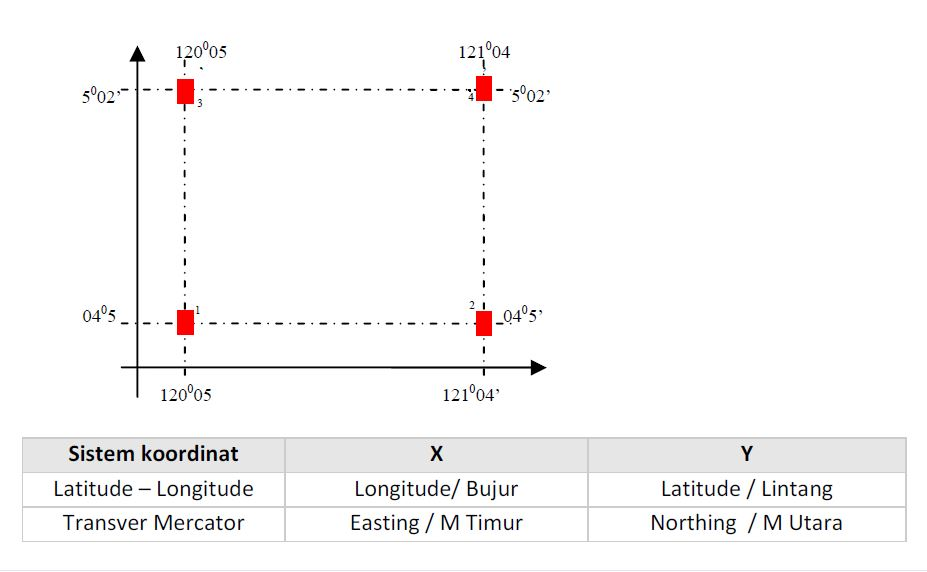
\includegraphics[width=4cm]{figures/1174063/koordinat.JPG}
	\centering
	\caption{Contoh Koordinat}
\end{figure}
Pada system koordinat UTM biasanya terdapat pembagian waktu berdasarkan zonasinya. \hfill\break
\begin{figure}[H]
	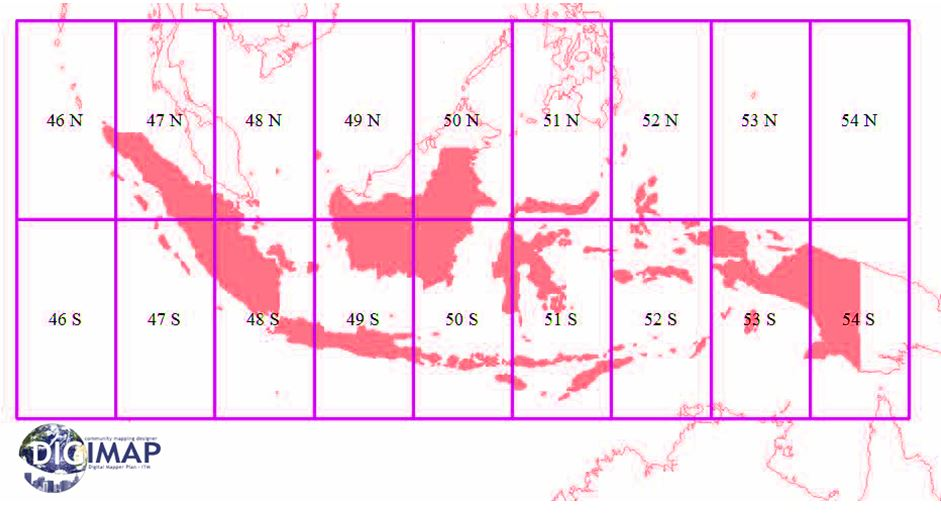
\includegraphics[width=4cm]{figures/1174063/utm.JPG}
	\centering
	\caption{Contoh Koordinat UTM}

	\subsection{Link}
\href{https://youtu.be/mU4dPSOHDWI}{LOOK AT THIS}
\subsection{Plagiarism}
\begin{figure}[H]
	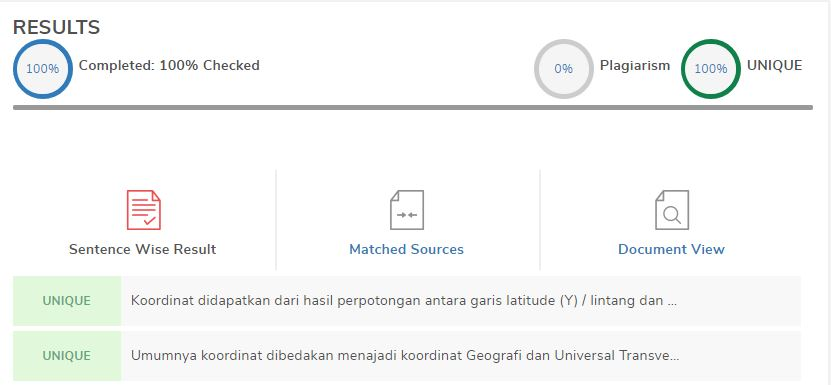
\includegraphics[width=4cm]{figures/1174063/plagiat.JPG}
	\centering
	\caption{Plagiat.}
\end{figure}


\input{chapters/tugas1/1174059}
\input{chapters/tugas1/1174038}
\section{Ichsan Hizman Hardy(1174034)}
\subsection{Membaca File PYSHP}
\begin{enumerate}
	\item 
	\lstinputlisting{src/2/1174034/1.py}
	\begin{figure}[H]
		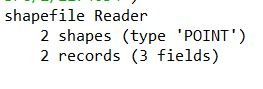
\includegraphics[width=12cm]{figures/1174034/tugas3/1.PNG}
		\centering
		\caption{Gambar no. 1}
	\end{figure}
	
	\item 
	\lstinputlisting{src/2/1174034/2.py}
	\begin{figure}[H]
		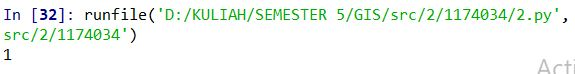
\includegraphics[width=12cm]{figures/1174034/tugas3/2.PNG}
		\centering
		\caption{Gambar no. 2}
	\end{figure}
	
	\item 
	\lstinputlisting{src/2/1174034/3.py}
	\begin{figure}[H]
		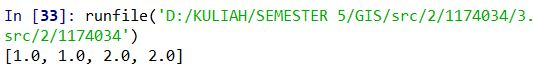
\includegraphics[width=12cm]{figures/1174034/tugas3/3.PNG}
		\centering
		\caption{Gambar no. 3}
	\end{figure}
	
	\item 
	\lstinputlisting{src/2/1174034/4.py}
	\begin{figure}[H]
		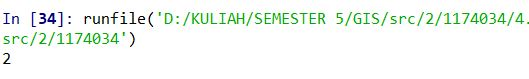
\includegraphics[width=12cm]{figures/1174034/tugas3/4.PNG}
		\centering
		\caption{Gambar no. 4}
	\end{figure}
	
	\item 
	\lstinputlisting{src/2/1174034/5.py}
	\begin{figure}[H]
		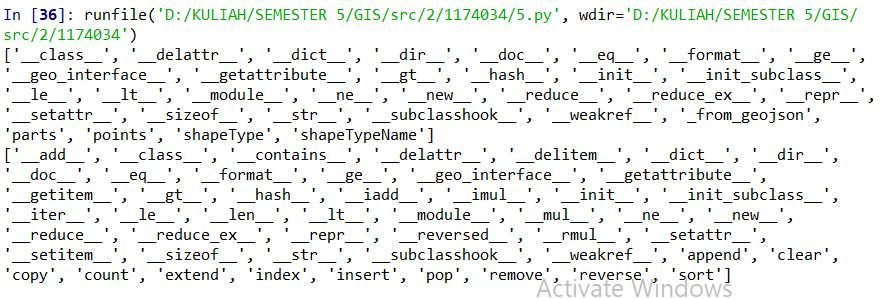
\includegraphics[width=12cm]{figures/1174034/tugas3/5.PNG}
		\centering
		\caption{Gambar no. 5}
	\end{figure}
	
	\item 
	\lstinputlisting{src/2/1174034/6.py}
	\begin{figure}[H]
		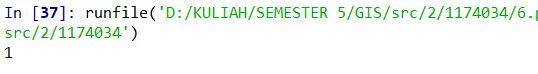
\includegraphics[width=12cm]{figures/1174034/tugas3/6.PNG}
		\centering
		\caption{Gambar no. 6}
	\end{figure}
	
	\item 
	\lstinputlisting{src/2/1174034/7.py}
	\begin{figure}[H]
		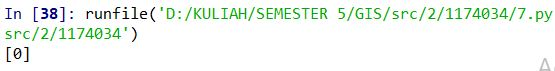
\includegraphics[width=12cm]{figures/1174034/tugas3/7.PNG}
		\centering
		\caption{Gambar no. 7}
	\end{figure}
	
	\item 
	\lstinputlisting{src/2/1174034/8.py}
	\begin{figure}[H]
		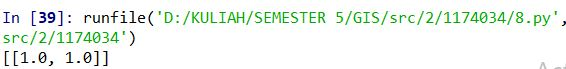
\includegraphics[width=12cm]{figures/1174034/tugas3/8.PNG}
		\centering
		\caption{Gambar no. 8}
	\end{figure}
	
	\item 
	\lstinputlisting{src/2/1174034/9.py}
	\begin{figure}[H]
		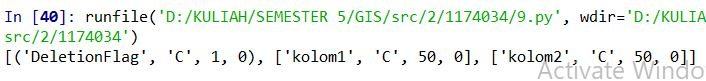
\includegraphics[width=12cm]{figures/1174034/tugas3/9.PNG}
		\centering
		\caption{Gambar no. 9}
	\end{figure}

    \item 
	\lstinputlisting{src/2/1174034/10.py}
	\begin{figure}[H]
		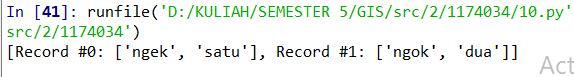
\includegraphics[width=12cm]{figures/1174034/tugas3/10.PNG}
		\centering
		\caption{Gambar no. 10}
	\end{figure}

	\item 
	\lstinputlisting{src/2/1174034/11.py}
	\begin{figure}[H]
		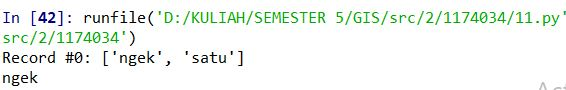
\includegraphics[width=12cm]{figures/1174034/tugas3/11.PNG}
		\centering
		\caption{Gambar no. 11}
	\end{figure}
\end{enumerate}

\subsection{Link}
\href{https://youtu.be/6CQ-dYhte20}{Youtubenya Ichsan Hizman}


\chapter{Tugas Kedua}
\input{chapters/tugas2/1174042}
\input{chapters/tugas2/1174040}
\input{chapters/tugas2/1174039}
\input{chapters/tugas2/1174043}
\input{chapters/tugas2/1174035}
\section{Dika Sukma Pradana(1174050)}
\subsection{LeafletJs bersama Map Proxy}
\begin{enumerate}
 \item Sesuaikan direktorinya dengan milik kita
    \hfill\break
    \begin{figure}[H]
		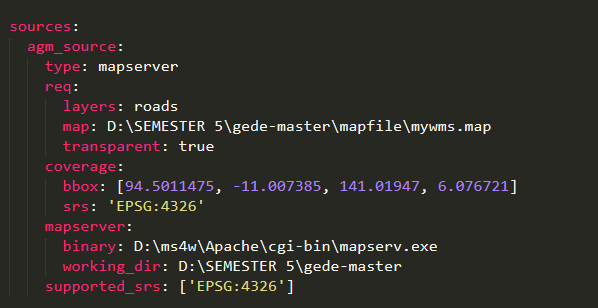
\includegraphics[width=12cm]{figures/1174050/tugas5/2.PNG}
		\centering
		\caption{Penyesuaian Direktori}
	\end{figure}
    \item Run Map Proxy dengan perintah mapproxy-util serve-develop agm.yaml
    \hfill\break
    \begin{figure}[H]
		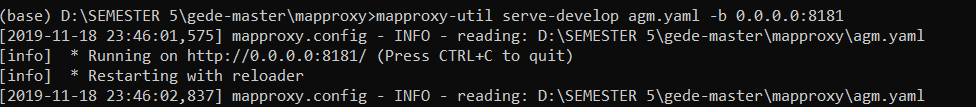
\includegraphics[width=12cm]{figures/1174050/tugas5/1.PNG}
		\centering
		\caption{Run MapProxy}
	\end{figure}
    \item Buka file basic.html di chrome sesuai direktorinya
    \hfill\break
    \begin{figure}[H]
		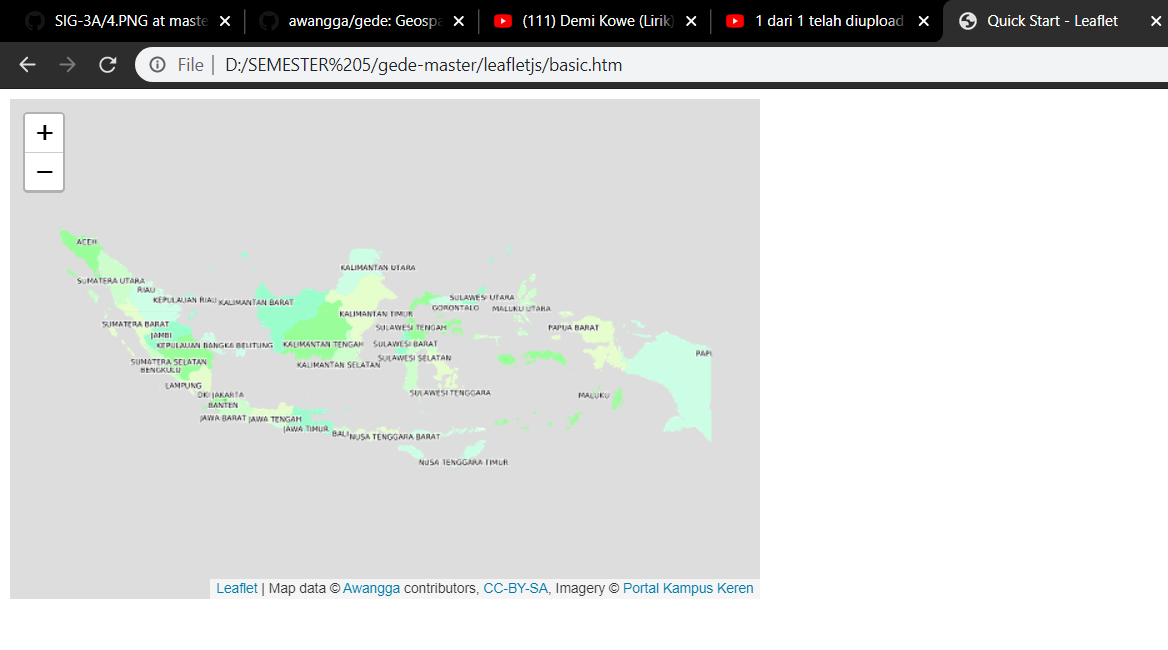
\includegraphics[width=12cm]{figures/1174050/tugas5/3.PNG}
		\centering
		\caption{Buka di Chrome}
	\end{figure}
    \item Pada file marker.html sudah ditambahkan marker pada daerah tertentu
    \hfill\break
    \begin{figure}[H]
		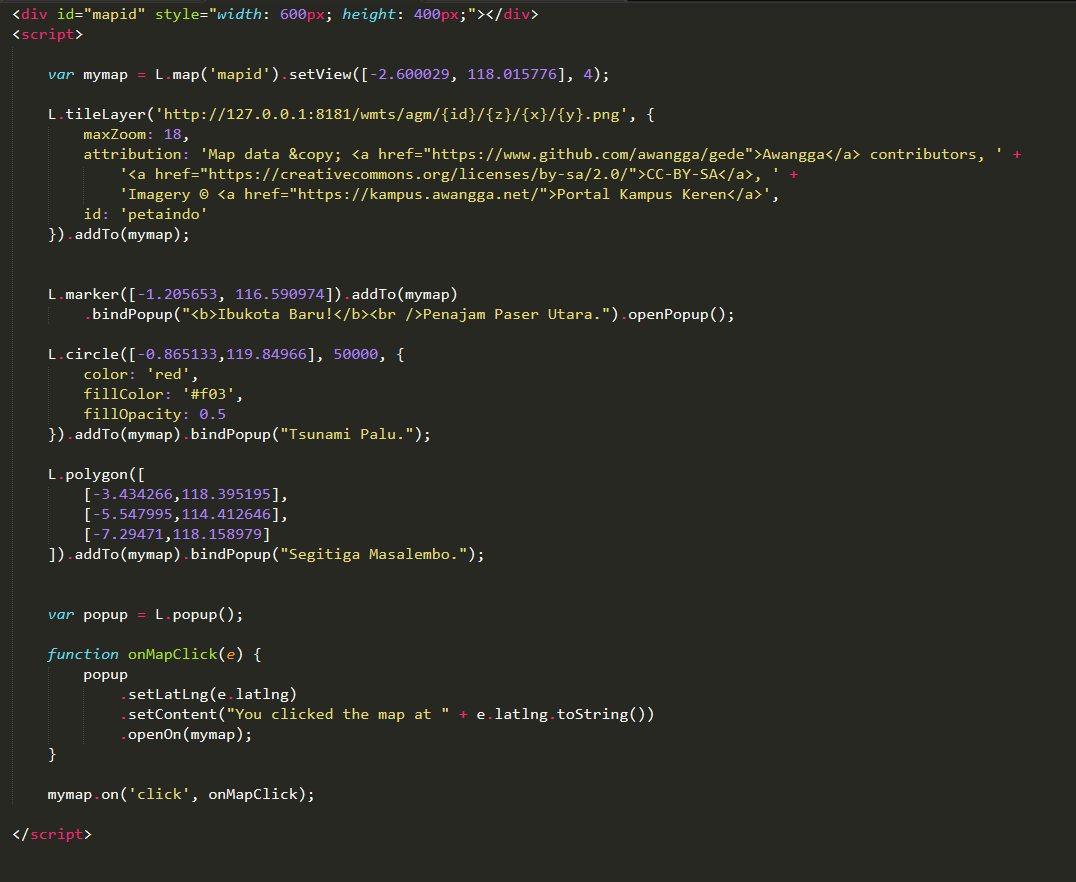
\includegraphics[width=12cm]{figures/1174050/tugas5/4.PNG}
		\centering
		\caption{Tambah Marker}
	\end{figure}
    \item Buka marker.html di browser
    \hfill\break
    \begin{figure}[H]
		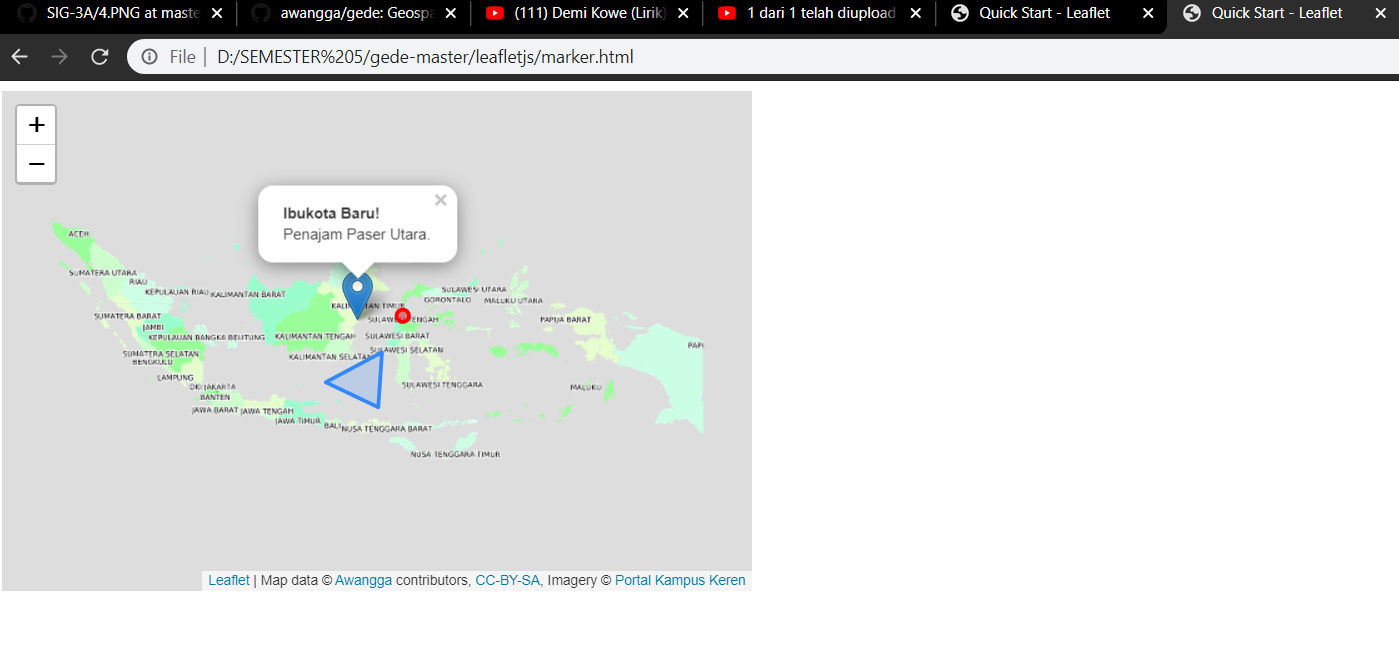
\includegraphics[width=12cm]{figures/1174050/tugas5/5.PNG}
		\centering
		\caption{Tampilan di Browser}
	\end{figure}
\end{enumerate}
\subsection{Link Youtube}
\href{https://youtu.be/1eIGj9vYuS4}{YOUTUBE!JANGAN LUPA SESKREB!}
\input{chapters/tugas2/1174059}
\input{chapters/tugas2/1174038}
\input{chapters/tugas2/1174056}
\section{Alit Fajar Kurniawan (1174057)}
\subsection{Membaca file shp dengan pyshp}
\begin{enumerate}
	\item 
	\lstinputlisting{src/2/1174057/soal1.py}
	\begin{figure}[H]
		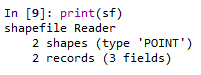
\includegraphics[width=12cm]{figures/1174057/fajar1.PNG}
		\centering
		\caption{Gambar no. 1}
	\end{figure}
	
	\item 
	\lstinputlisting{src/2/1174057/soal2.py}
	\begin{figure}[H]
		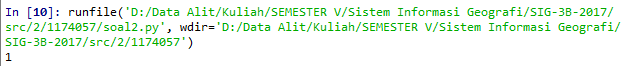
\includegraphics[width=12cm]{figures/1174057/fajar2.PNG}
		\centering
		\caption{Gambar no. 2}
	\end{figure}
	
	\item 
	\lstinputlisting{src/2/1174057/soal3.py}
	\begin{figure}[H]
		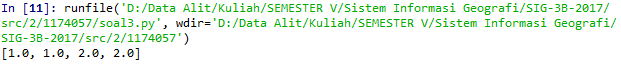
\includegraphics[width=12cm]{figures/1174057/fajar3.PNG}
		\centering
		\caption{Gambar no. 3}
	\end{figure}
	
	\item 
	\lstinputlisting{src/2/1174057/soal4.py}
	\begin{figure}[H]
		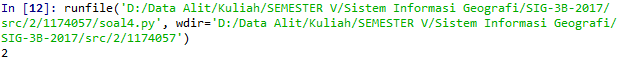
\includegraphics[width=12cm]{figures/1174057/fajar4.PNG}
		\centering
		\caption{Gambar no. 4}
	\end{figure}
	
	\item 
	\lstinputlisting{src/2/1174057/soal5.py}
	\begin{figure}[H]
		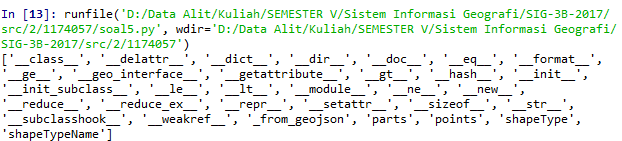
\includegraphics[width=12cm]{figures/1174057/fajar5.PNG}
		\centering
		\caption{Gambar no. 5}
	\end{figure}
	
	\item 
	\lstinputlisting{src/2/1174057/soal6.py}
	\begin{figure}[H]
		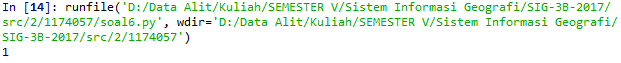
\includegraphics[width=12cm]{figures/1174057/fajar6.PNG}
		\centering
		\caption{Gambar no. 6}
	\end{figure}
	
	\item 
	\lstinputlisting{src/2/1174057/soal7.py}
	\begin{figure}[H]
		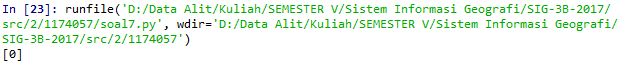
\includegraphics[width=12cm]{figures/1174057/fajar7.PNG}
		\centering
		\caption{Gambar no. 7}
	\end{figure}
	
	\item 
	\lstinputlisting{src/2/1174040/8.py}
	\begin{figure}[H]
		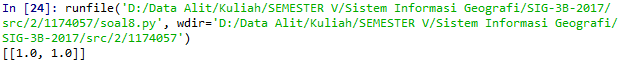
\includegraphics[width=12cm]{figures/1174057/fajar8.PNG}
		\centering
		\caption{Gambar no. 8}
	\end{figure}
	
	\item 
	\lstinputlisting{src/2/1174057/soal9.py}
	\begin{figure}[H]
		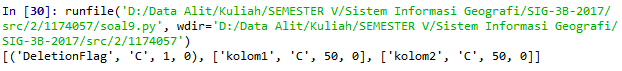
\includegraphics[width=12cm]{figures/1174057/fajar9.PNG}
		\centering
		\caption{Gambar no. 9}
	\end{figure}

    \item 
	\lstinputlisting{src/2/1174057/soal10.py}
	\begin{figure}[H]
		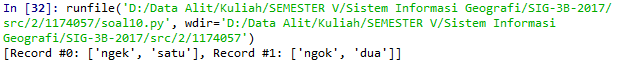
\includegraphics[width=12cm]{figures/1174057/fajar10.PNG}
		\centering
		\caption{Gambar no. 10}
	\end{figure}

	\item 
	\lstinputlisting{src/2/1174057/soal11.py}
	\begin{figure}[H]
		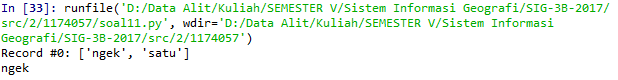
\includegraphics[width=12cm]{figures/1174057/fajar11.PNG}
		\centering
		\caption{Gambar no. 11}
	\end{figure}
\end{enumerate}

\subsection{Link}
\href{https://www.youtube.com/watch?v=PxCZFZzLivM}{Video ni}
\section{Ichsan Hizman Hardy(1174034)}
\subsection{Membaca File PYSHP}
\begin{enumerate}
	\item 
	\lstinputlisting{src/2/1174034/1.py}
	\begin{figure}[H]
		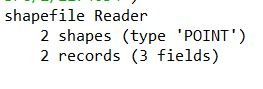
\includegraphics[width=12cm]{figures/1174034/tugas3/1.PNG}
		\centering
		\caption{Gambar no. 1}
	\end{figure}
	
	\item 
	\lstinputlisting{src/2/1174034/2.py}
	\begin{figure}[H]
		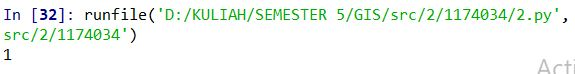
\includegraphics[width=12cm]{figures/1174034/tugas3/2.PNG}
		\centering
		\caption{Gambar no. 2}
	\end{figure}
	
	\item 
	\lstinputlisting{src/2/1174034/3.py}
	\begin{figure}[H]
		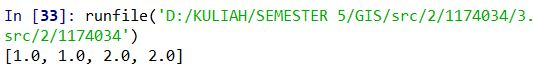
\includegraphics[width=12cm]{figures/1174034/tugas3/3.PNG}
		\centering
		\caption{Gambar no. 3}
	\end{figure}
	
	\item 
	\lstinputlisting{src/2/1174034/4.py}
	\begin{figure}[H]
		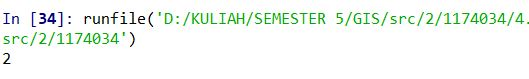
\includegraphics[width=12cm]{figures/1174034/tugas3/4.PNG}
		\centering
		\caption{Gambar no. 4}
	\end{figure}
	
	\item 
	\lstinputlisting{src/2/1174034/5.py}
	\begin{figure}[H]
		\includegraphics[width=12cm]{figures/1174034/tugas3/5.PNG}
		\centering
		\caption{Gambar no. 5}
	\end{figure}
	
	\item 
	\lstinputlisting{src/2/1174034/6.py}
	\begin{figure}[H]
		\includegraphics[width=12cm]{figures/1174034/tugas3/6.PNG}
		\centering
		\caption{Gambar no. 6}
	\end{figure}
	
	\item 
	\lstinputlisting{src/2/1174034/7.py}
	\begin{figure}[H]
		\includegraphics[width=12cm]{figures/1174034/tugas3/7.PNG}
		\centering
		\caption{Gambar no. 7}
	\end{figure}
	
	\item 
	\lstinputlisting{src/2/1174034/8.py}
	\begin{figure}[H]
		\includegraphics[width=12cm]{figures/1174034/tugas3/8.PNG}
		\centering
		\caption{Gambar no. 8}
	\end{figure}
	
	\item 
	\lstinputlisting{src/2/1174034/9.py}
	\begin{figure}[H]
		\includegraphics[width=12cm]{figures/1174034/tugas3/9.PNG}
		\centering
		\caption{Gambar no. 9}
	\end{figure}

    \item 
	\lstinputlisting{src/2/1174034/10.py}
	\begin{figure}[H]
		\includegraphics[width=12cm]{figures/1174034/tugas3/10.PNG}
		\centering
		\caption{Gambar no. 10}
	\end{figure}

	\item 
	\lstinputlisting{src/2/1174034/11.py}
	\begin{figure}[H]
		\includegraphics[width=12cm]{figures/1174034/tugas3/11.PNG}
		\centering
		\caption{Gambar no. 11}
	\end{figure}
\end{enumerate}

\subsection{Link}
\href{https://youtu.be/6CQ-dYhte20}{Youtubenya Ichsan Hizman}
\section{MuhammadIqbalPanggabean(1174063)}

\subsection{Koordinat}
Koordinat didapatkan dari hasil perpotongan antara garis latitude (Y) / lintang dan garis longitude(X) / garis bujur sehingga bisa menunjukan suatu lokasi pada suatu daerah. \hfill\break 
Umumnya koordinat dibedakan menajadi koordinat Geografi dan Universal Transver Mercator(UTM). Pada koordinat geografi dibedakan menajadi 3 yaitu : \hfill\break
\begin{itemize}
	\item Degree, Decimal(DD, DDDD) contoh S 4.56734 E 102.67235
	\item Degree,Minute(DD MM,MMMM) contoh S 4 42,5423’ E 105 34,6445’
	\item Degree, Minute, Second(DD MM SS,SS) contoh : S 4 43’ 45,22 E 103 33’ 33,25
\end{itemize}
\hfill\break
\begin{figure}[H]
	\includegraphics[width=4cm]{figures/1174063/koordinat.JPG}
	\centering
	\caption{Contoh Koordinat}
\end{figure}
Pada system koordinat UTM biasanya terdapat pembagian waktu berdasarkan zonasinya. \hfill\break
\begin{figure}[H]
	\includegraphics[width=4cm]{figures/1174063/utm.JPG}
	\centering
	\caption{Contoh Koordinat UTM}

	\subsection{Link}
\href{https://youtu.be/mU4dPSOHDWI}{LOOK AT THIS}
\subsection{Plagiarism}
\begin{figure}[H]
	\includegraphics[width=4cm]{figures/1174063/plagiat.JPG}
	\centering
	\caption{Plagiat.}
\end{figure}




\chapter{Tugas Ketiga}
\input{chapters/tugas3/1174039}
\input{chapters/tugas3/1174043}
\input{chapters/tugas3/1174035}
\input{chapters/tugas3/1174040}
\section{Dika Sukma Pradana 1174050)}
\subsection{Membaca File PYSHP}
\begin{enumerate}
    \item 
    \lstinputlisting{src/2/1174050/1.py}
    \begin{figure}[H]
		\includegraphics[width=6cm]{figures/1174050/Tugas3/1.png}
		\centering
		\caption{Nomor 1}
	\end{figure}
    \item 
    \lstinputlisting{src/2/1174050/2.py}
    \begin{figure}[H]
		\includegraphics[width=6cm]{figures/1174050/Tugas3/2.png}
		\centering
		\caption{Nomor 2}
    \end{figure}
    \item 
    \lstinputlisting{src/2/1174050/3.py}
    \begin{figure}[H]
		\includegraphics[width=6cm]{figures/1174050/Tugas3/3.png}
		\centering
		\caption{Nomor 3}
    \end{figure}
    \item 
    \lstinputlisting{src/2/1174050/4.py}
    \begin{figure}[H]
		\includegraphics[width=6cm]{figures/1174050/Tugas3/4.png}
		\centering
		\caption{Nomor 4}
    \end{figure}
    \item 
    \lstinputlisting{src/2/1174050/5.py}
    \begin{figure}[H]
		\includegraphics[width=6cm]{figures/1174050/Tugas3/5.png}
		\centering
		\caption{Nomor 5}
    \end{figure}
    \item 
    \lstinputlisting{src/2/1174050/6.py}
    \begin{figure}[H]
		\includegraphics[width=6cm]{figures/1174050/Tugas3/6.png}
		\centering
		\caption{Nomor 6}
    \end{figure}
    \item 
    \lstinputlisting{src/2/1174050/7.py}
    \begin{figure}[H]
		\includegraphics[width=6cm]{figures/1174050/Tugas3/7.png}
		\centering
		\caption{Nomor 7}
    \end{figure}
    \item 
    \lstinputlisting{src/2/1174050/8.py}
    \begin{figure}[H]
		\includegraphics[width=6cm]{figures/1174050/Tugas3/8.png}
		\centering
		\caption{Nomor 8}
    \end{figure}
    \item 
    \lstinputlisting{src/2/1174050/9.py}
    \begin{figure}[H]
		\includegraphics[width=6cm]{figures/1174050/Tugas3/9.png}
		\centering
		\caption{Nomor 9}
    \end{figure}
    \item 
    \lstinputlisting{src/2/1174050/10.py}
    \begin{figure}[H]
		\includegraphics[width=6cm]{figures/1174050/Tugas3/10.png}
		\centering
		\caption{Nomor 10}
    \end{figure}
    \item 
    \lstinputlisting{src/2/1174050/11.py}
    \begin{figure}[H]
		\includegraphics[width=6cm]{figures/1174050/Tugas3/11.png}
		\centering
		\caption{Nomor 11}
	\end{figure}
\end{enumerate}
\subsection{Link Youtube}
\href{https://youtu.be/-_xwZFC9QGE}{Youtube! JANGAN LUPA SESKREB!}
\section{Ichsan Hizman Hardy(1174034)}
\subsection{Membaca File PYSHP}
\begin{enumerate}
	\item 
	\lstinputlisting{src/2/1174034/1.py}
	\begin{figure}[H]
		\includegraphics[width=12cm]{figures/1174034/tugas3/1.PNG}
		\centering
		\caption{Gambar no. 1}
	\end{figure}
	
	\item 
	\lstinputlisting{src/2/1174034/2.py}
	\begin{figure}[H]
		\includegraphics[width=12cm]{figures/1174034/tugas3/2.PNG}
		\centering
		\caption{Gambar no. 2}
	\end{figure}
	
	\item 
	\lstinputlisting{src/2/1174034/3.py}
	\begin{figure}[H]
		\includegraphics[width=12cm]{figures/1174034/tugas3/3.PNG}
		\centering
		\caption{Gambar no. 3}
	\end{figure}
	
	\item 
	\lstinputlisting{src/2/1174034/4.py}
	\begin{figure}[H]
		\includegraphics[width=12cm]{figures/1174034/tugas3/4.PNG}
		\centering
		\caption{Gambar no. 4}
	\end{figure}
	
	\item 
	\lstinputlisting{src/2/1174034/5.py}
	\begin{figure}[H]
		\includegraphics[width=12cm]{figures/1174034/tugas3/5.PNG}
		\centering
		\caption{Gambar no. 5}
	\end{figure}
	
	\item 
	\lstinputlisting{src/2/1174034/6.py}
	\begin{figure}[H]
		\includegraphics[width=12cm]{figures/1174034/tugas3/6.PNG}
		\centering
		\caption{Gambar no. 6}
	\end{figure}
	
	\item 
	\lstinputlisting{src/2/1174034/7.py}
	\begin{figure}[H]
		\includegraphics[width=12cm]{figures/1174034/tugas3/7.PNG}
		\centering
		\caption{Gambar no. 7}
	\end{figure}
	
	\item 
	\lstinputlisting{src/2/1174034/8.py}
	\begin{figure}[H]
		\includegraphics[width=12cm]{figures/1174034/tugas3/8.PNG}
		\centering
		\caption{Gambar no. 8}
	\end{figure}
	
	\item 
	\lstinputlisting{src/2/1174034/9.py}
	\begin{figure}[H]
		\includegraphics[width=12cm]{figures/1174034/tugas3/9.PNG}
		\centering
		\caption{Gambar no. 9}
	\end{figure}

    \item 
	\lstinputlisting{src/2/1174034/10.py}
	\begin{figure}[H]
		\includegraphics[width=12cm]{figures/1174034/tugas3/10.PNG}
		\centering
		\caption{Gambar no. 10}
	\end{figure}

	\item 
	\lstinputlisting{src/2/1174034/11.py}
	\begin{figure}[H]
		\includegraphics[width=12cm]{figures/1174034/tugas3/11.PNG}
		\centering
		\caption{Gambar no. 11}
	\end{figure}
\end{enumerate}

\subsection{Link}
\href{https://youtu.be/6CQ-dYhte20}{Youtubenya Ichsan Hizman}
\section{Alit Fajar Kurniawan (1174057)}
\subsection{Membaca file shp dengan pyshp}
\begin{enumerate}
	\item 
	\lstinputlisting{src/2/1174057/soal1.py}
	\begin{figure}[H]
		\includegraphics[width=12cm]{figures/1174057/fajar1.PNG}
		\centering
		\caption{Gambar no. 1}
	\end{figure}
	
	\item 
	\lstinputlisting{src/2/1174057/soal2.py}
	\begin{figure}[H]
		\includegraphics[width=12cm]{figures/1174057/fajar2.PNG}
		\centering
		\caption{Gambar no. 2}
	\end{figure}
	
	\item 
	\lstinputlisting{src/2/1174057/soal3.py}
	\begin{figure}[H]
		\includegraphics[width=12cm]{figures/1174057/fajar3.PNG}
		\centering
		\caption{Gambar no. 3}
	\end{figure}
	
	\item 
	\lstinputlisting{src/2/1174057/soal4.py}
	\begin{figure}[H]
		\includegraphics[width=12cm]{figures/1174057/fajar4.PNG}
		\centering
		\caption{Gambar no. 4}
	\end{figure}
	
	\item 
	\lstinputlisting{src/2/1174057/soal5.py}
	\begin{figure}[H]
		\includegraphics[width=12cm]{figures/1174057/fajar5.PNG}
		\centering
		\caption{Gambar no. 5}
	\end{figure}
	
	\item 
	\lstinputlisting{src/2/1174057/soal6.py}
	\begin{figure}[H]
		\includegraphics[width=12cm]{figures/1174057/fajar6.PNG}
		\centering
		\caption{Gambar no. 6}
	\end{figure}
	
	\item 
	\lstinputlisting{src/2/1174057/soal7.py}
	\begin{figure}[H]
		\includegraphics[width=12cm]{figures/1174057/fajar7.PNG}
		\centering
		\caption{Gambar no. 7}
	\end{figure}
	
	\item 
	\lstinputlisting{src/2/1174040/8.py}
	\begin{figure}[H]
		\includegraphics[width=12cm]{figures/1174057/fajar8.PNG}
		\centering
		\caption{Gambar no. 8}
	\end{figure}
	
	\item 
	\lstinputlisting{src/2/1174057/soal9.py}
	\begin{figure}[H]
		\includegraphics[width=12cm]{figures/1174057/fajar9.PNG}
		\centering
		\caption{Gambar no. 9}
	\end{figure}

    \item 
	\lstinputlisting{src/2/1174057/soal10.py}
	\begin{figure}[H]
		\includegraphics[width=12cm]{figures/1174057/fajar10.PNG}
		\centering
		\caption{Gambar no. 10}
	\end{figure}

	\item 
	\lstinputlisting{src/2/1174057/soal11.py}
	\begin{figure}[H]
		\includegraphics[width=12cm]{figures/1174057/fajar11.PNG}
		\centering
		\caption{Gambar no. 11}
	\end{figure}
\end{enumerate}

\subsection{Link}
\href{https://www.youtube.com/watch?v=PxCZFZzLivM}{Video ni}

\bibliographystyle{IEEEtran}
%\def\bibfont{\normalsize}
\bibliography{references}
%%%%%%%%%%%%%%%%%%%%%%%%%%%%%%%%%%%%%%%%%%%%%%


%%%%%%%%%%%%%%%
%%  The default LaTeX Index
%%  Don't need to add any commands before \begin{document}
\printindex

%%%% Making an index
%%
%% 1. Make index entries, don't leave any spaces so that they
%% will be sorted correctly.
%%
%% \index{term}
%% \index{term!subterm}
%% \index{term!subterm!subsubterm}
%%
%% 2. Run LaTeX several times to produce <filename>.idx
%%
%% 3. On command line, type  makeindx <filename> which
%% will produce <filename>.ind
%%
%% 4. Type \printindex to make the index appear in your book.
%%
%% 5. If you would like to edit <filename>.ind
%% you may do so. See docs.pdf for more information.
%%
%%%%%%%%%%%%%%%%%%%%%%%%%%%%%%

%%%%%%%%%%%%%% Making Multiple Indices %%%%%%%%%%%%%%%%
%% 1.
%% \usepackage{multind}
%% \makeindex{book}
%% \makeindex{authors}
%% \begin{document}
%%
%% 2.
%% % add index terms to your book, ie,
%% \index{book}{A term to go to the topic index}
%% \index{authors}{Put this author in the author index}
%%
%% \index{book}{Cows}
%% \index{book}{Cows!Jersey}
%% \index{book}{Cows!Jersey!Brown}
%%
%% \index{author}{Douglas Adams}
%% \index{author}{Boethius}
%% \index{author}{Mark Twain}
%%
%% 3. On command line type
%% makeindex topic
%% makeindex authors
%%
%% 4.
%% this is a Wiley command to make the indices print:
%% \multiprintindex{book}{Topic index}
%% \multiprintindex{authors}{Author index}

\end{document}

